\documentclass[a4paper, 11pt]{llncs}

%\documentclass[conference]{IEEEtran}
%\IEEEoverridecommandlockouts

\usepackage{amsmath,amssymb}
\usepackage{stmaryrd}
\usepackage{tikz}
\usepackage{url}
\usetikzlibrary{automata, positioning, arrows}
\usepackage{array}
%\ifCLASSOPTIONcompsoc
% requires cite.sty v4.0 or later (November 2003)
%\usepackage[nocompress]{cite}
%\else
%\usepackage{cite}
%\fi

%% Macros

% Greek
%\newtheorem{definition}{Definition}


%\newtheorem{example}{Example}
%\newtheorem{lemma}{Lemma}
%\newtheorem{corollary}{Corollary}
%\newtheorem{proof}{IEEEproof}
%\newtheorem{theorem}{Theorem}

\renewcommand{\a}{\alpha}
\renewcommand{\b}{\beta}
\newcommand{\s}{\sigma}
\renewcommand{\d}{\delta}
\newcommand{\e}{\epsilon}
\newcommand{\m}{\mu}

\newcommand{\D}{\Delta}

\newcommand{\rr}{\mathsf{r}}
\newcommand{\bb}{\mathsf{b}}
\renewcommand{\gg}{\mathsf{g}}
\newcommand{\yy}{\mathsf{y}}
\newcommand{\ww}{\mathsf{w}}
% Mathcal
\newcommand{\Aa}{\mathcal{A}}
\newcommand{\Ll}{\mathcal{L}}
\newcommand{\Oo}{\mathcal{O}}
\newcommand{\Ss}{\mathcal{S}}
\newcommand{\Ww}{\mathcal{W}}
% Symbols
\newcommand{\imp}{\Rightarrow}
\newcommand{\xra}{\xrightarrow}
\newcommand{\Land}{\bigwedge}
\newcommand{\incl}{\subseteq}

% Misc
\newcommand{\ssczo}{C_{0 \to 1}}
\newcommand{\coz}{C_{1 \to 0}}
\newcommand{\sem}[1]{\llbracket #1 \rrbracket}
%\renewcommand{\sp}{\operatorname{SP}}
%\renewcommand{\sp}{\sigma}
\renewcommand{\sp}{\mathcal{S}\mathcal{L}}
\newcommand{\context}{\mathcal{C}}
\newcommand{\border}{\mathcal{B}}
\newcommand{\nbd}{(\mathcal{C} + \mathcal{B})}
\newcommand{\prfx}{\sqsubseteq_{\mathsf {pr}}}
\newcommand{\pprfx}{\sqsubset_{\mathsf {pr}}}
\newcommand{\sfx}{\sqsubseteq_{\mathsf {sf}}}
\newcommand{\psfx}{\sqsubset_{\mathsf {sf}}}
\newcommand{\proj}[1]{\mathsf{P}_{#1}}
\newcommand{\spm}{\sp^{\mathsf{m}}}
\newcommand{\sfxm}{\sfx^{\mathsf{m}}}
\newcommand{\psfxm}{\psfx^{\mathsf{m}}}
%\renewcommand{\IEEEQED}{\IEEEQEDopen}

\newcommand{\PSPACE}{\operatorname{\textsc{Pspace}}}
\newcommand{\NP}{\mathsf{NP}}
\newcommand{\coNP}{\mathsf{coNP}}
\newcommand{\vertex}{\textsc{VertexCover}~}
\newcommand{\mdsa}{DSA$^{\mathsf{m}}$}

\newcommand{\out}{\operatorname{Out}}
\newcommand{\outp}{\operatorname{Out}_{\sqsubset}}

\newcommand{\lsfx}[1]{\sqsubseteq_{\scriptscriptstyle
    \mathsf{lsf}}^{\scriptscriptstyle #1}}
\newcommand{\sub}{\sqsubseteq_{\mathsf{sub}}}
\newcommand{\rsub}{\sqsubset_{\mathsf{sub}^{\mathsf{r}}}}
\renewcommand{\e}{\varepsilon}
\renewcommand{\epsilon}{\e}

\newcommand{\Tt}{\mathcal{T}}
\newcommand{\Ii}{\mathcal{I}}
\newcommand{\Vv}{\mathcal{V}}
%\input{macros}
\newcommand{\specialcell}[2][c]{%
  \begin{tabular}[#1]{@{}c@{}}#2\end{tabular}}
\newcommand{\var}{\operatorname{Var}}
\newcommand{\dom}{\ensuremath{dom}}


\begin{document}
\title{Suffix-reading automata in a practical setting}

\maketitle

\label{sec:multi-port-inputs}%


Consider a special kind of an alphabet
$\Sigma = \langle \Sigma_1, \Sigma_2, \dots, \Sigma_k \rangle$ such
that $\Sigma_i \cap \Sigma_j = \emptyset$ for all $i, j \in
[1..k]$. We will call $\Sigma_i$ as the alphabet of \emph{port} $i$,
and $\Sigma$ as a \emph{multi-port} alphabet. We
look at DFAs over such multi-port alphabets. Such DFAs model systems
that listen to inputs from different processes and perform actions
based on them. Sometimes the order in which the system receives its
inputs from different ports is not relevant.%
  
For example, at a state
$s$, if the system receives $a$ from port 1 and $b$ from port 2, in any
order, then it has to go to state $t$.  A DFA would model this with
transitions: $s \xra{a} s_a \xra{b} t$ and $s \xra{b} s_b \xra{a}
t$. A DSA would contain two transitions $s \xra{ab, ba} t$ (and some
other transitions, if needed, to take care of $aa$, $bb$). To get a
more succinct notation we will use a $\parallel$ operator. We will
write $s \xra{a \parallel b} t$ to mean that at state $s$, when
both $a$ and $b$ are received, the automaton moves to $t$. When there
are several components, this notation leads to significant
succinctness, for instance $a_1 \parallel a_2 \cdots \parallel a_n$
stands for all the $n!$ permutations of $a_1$ to $a_n$. We will also
allow expressions of the form $a_1 a_2 \parallel b$, which stands for
the set of words $\{a_1 a_2 b, a_1 b a_2, b a_1 a_2\}$ which shuffles
$a_1a_2$ and $b$. We will now formalize this idea by enhancing DSA with
the $\parallel$ operator and then consider the problem of synthesizing
such extended DSA. We begin with some notation.%

% DFAs model
% a system consisting of $k$-components, where the $i^{th}$ component
% has sole control over actions of $\Sigma_i$. However every component
% can observe the actions generated by all other components. So, instead
% of modeling such a system as a network of automata, we consider it to
% be a single DFA over this multi-port alphabet. Therefore, for a start, 
% there is no ``independence'' between the ports: for example if
% action $a$ is controlled by process $1$ and action $b$ is controlled
% by process $2$, we cannot in general commute the sequence $ab$ with
% $ba$: it may be the case that process $2$ waits for process $1$ to
% emit an $a$. However, in the DFA, there could be
% specific parts where there is independence, in other words, there are
% states $s$, $t$ and a set of actions coming from different ports such
% that all interleavings among different ports are possible between $s$
% and $t$. We wish to extend the definition of a suffix-reading
% automaton with the aim to capture more succinctly these ``diamonds'' occurring in the
% DFA. %



\paragraph*{Notation} For a word $w \in \Sigma^*$, we write
$\proj{i}(w)$ for the projection of $w$ onto the set $\Sigma_i$. For
instance, if $\Sigma_1 = \{a_1, a_2\}, \Sigma_2 = \{b_1, b_2\}$ and
$w = a_1 b_1 a_2 a_1 b_2 b_2$, we have $\proj{1}(w) = a_1 a_2 a_1$ and
$\proj{2}{w} = b_1 b_2 b_2$.  We write $\partial w$ for the $k$-tuple
$(\proj{1}(w), \proj{2}(w), \dots, \proj{k}(w))$ of projections of $w$
onto each port $\Sigma_i$, and will call $\partial w$ the
\emph{decomposition} of $w$. Notice that if
$\partial w_1 = \partial w_2$ for two words $w_1, w_2$, then $w_1$ and
$w_2$ have the same order of events within each port, but could have a
different ordering between letters from different ports.%


\begin{definition} Let
 $\Sigma = \langle \Sigma_1, \Sigma_2, \dots, \Sigma_k \rangle$ be a
 multi-port alphabet. A \emph{multi-port (deterministic)
   suffix-reading automaton} (written \mdsa in short) $\Aa$ is a
 tuple $(Q, \Sigma, q^{init}, \delta, F)$ where $Q$, $q^{init}$ and
 $F$ are a finite set of states, the initial state and a set of
 accept states, respectively. The transition relation
 $\d \incl Q \times (\Sigma_1^* \times \Sigma_2^* \times \cdots
 \times \Sigma_k^*) \times Q$: each transition is of the form
 $(q, (u_1 \parallel u_2 \parallel \cdots \parallel u_k), q')$ where
 $u_i \in \Sigma_i^*$ (not all of them can be $\epsilon$).
 % We assume that for every two outgoing
 % transitions
 % $(q, (u_1, u_2, \dots, u_k), q_1)$ and
 % $(q, (v_1, v_2, \dots, v_k), q_2)$ there is at least one port $i$
 % such that $u_i$ and $v_i$ are suffix-incomparable, that is,
 % $u_i \not \sfx v_i$ and $v_i \not \sfx u_i$.
\end{definition}%

%\textcolor{red}{Jan 10, 2023. The first instinct is to say that the
% transition $q \xra{u_1 \parallel u_2 \cdots u_k} q'$ can be replaced
% with multiple transitions to get the usual DSA of the previous
% section. For instance $q \xra{a \parallel b} q'$ can be replaced
% with $q \xra{ab} q'$ and $q \xra{ba} q'$. But this is not correct in
% general!
% Suppose there is a third port. Consider a transition
% $q \xra{a \parallel b \parallel \epsilon} q'$. The third $\epsilon$
% is to say that we do not care what happens in that port. It does not mean
% that there is no input! We cannot just replace it with $\xra{ab}$
% and $\xra{ba}$. If we do so, the word $a c b$ at state $q$ would not
% move
% to $q'$ ($c$ is in third port), whereas it should. In fact, we
% cannot replace it with finitely many transitions: $a w b$ with $w$ a
% word using the third port alphabet is good for $a \parallel b
% \parallel \epsilon$. So, we need a completely fresh analysis for extending
% the parallel operation to DSA. We could keep this for future work.}%

\paragraph*{Semantics} $B=\langle B_1,B_2,\dots,B_{k'} \rangle$ is a tuple of tapes, one for each port and some additional ones ($k'\ge k$). Each tape has several tape heads, one for each unique transition label (corresponding to a `system requirement'), that track the previous `match' for each such requirement. 

\begin{enumerate}
\item All tapes are initially empty, with all the tape heads at zero. (call the head positions for the $B_i$ tape tracking transition label $j$, $H_{i}^{j}$)

\item When an input $a \in \Sigma_i$ is seen, the tape $B_i$ extends right by one position and store the value $a$.

\item A transition $(q, (u_1 \parallel u_2 \parallel \cdots \parallel u_k), q')$ with label $j$ (that is $u_1 \parallel u_2 \parallel \cdots \parallel u_k$) is \emph{matched} if every $B_i$ has $u_i$ as a suffix of its stored word, with either $H_{i}^{j}$ at the end of the tape or the entire $u_i$ present after $H_{i}^{j}$. Additionally, at least one $B_i$ has $H_{i}^{j}$ not at the end of the tape.

\item A matched transition is then \emph{triggered}, that is $\forall u_i \ne \epsilon$, the $H_{i}^{j}$ moves to the end. 
\end{enumerate}

The states of a multi-port DSA are defined as per the requirements of the system it models. For a system with internal variables $S_1,S_2,\dots$ with each variable $S_i$ having an alphabet $\Sigma_{S_i}$, the corresponding \mdsa has states $Q=\Sigma_1 \times \Sigma_2 \times \dots$. The additional tapes $B_{k+1}, B_{k+2}, \dots, B_{k'}$ are for the internal variables used in the system. These variables can read input as well as produce output, over the common alphabet representing their state space. %For example, a variable $S_i$ has an alphabet $\Sigma_{S_i}$ with letters that can be input as well as output.

Transitions must then be enhanced in our semantics i.e.  a transition $(q, (u_1, \dots, u_k), q')$ can now require the local variables $S_1, S_2,\dots$ to have values $(s_1, s_2 \dots)$  for it to match. When triggered, the values then change to $(s'_1,s'_2,\dots)$. Assume each variable $S_i$ has its corresponding tape labeled $B_{S_i}$ (we relabel the tapes $B_{k+1}, B_{k+2}, \dots, B_{k'}$ appropriately). Let us use the syntax $\langle (q, (s_1, s_2 \dots), (u_1, \dots, u_k), (s'_1,s'_2,\dots), q') \rangle$ to represent this.

\begin{enumerate}
\item A transition (with label $j$) $\langle (q, (s_1, s_2 \dots), (u_1, \dots, u_k), (s'_1,s'_2,\dots), q') \rangle$ is matched if each $B_i (i\le k)$ has $u_i$ as suffix, the last letter of each $B_{S_i}$ is $s_i$, and either $H_{i}^{j}$ is at the end or the entire $u_i$ is after $H_{i}^{j}$. Additionally, at least one tape is non-empty after $H_{i}^{j}$.

\item A matched transition is then triggered, moving each $H_{i}^{j}$-head of $B_i$ (or $B_{S_i}$) to the end $\forall u_i \ne \epsilon$ and $\forall s_i \ne \epsilon$. Additionally $\forall s'_i \ne \epsilon$, the corresponding $B_{S_i}$ extends by one position to the right and stores $s'_i$.
\end{enumerate}

% Given states $q, q'$, we say that a word $w \in \Sigma^*$ matches a
% transition $(q, (u_1, \dots, u_k), q')$ at $q$ if
% $u_i \sfx \proj{i}(w)$ for all $i$. When the automaton is in state
% $q$ and reads a word $w$, we say that transition
% $\theta = (q, (u_1, \dots, u_k), q')$ is \emph{triggered} if $w$
% matches $\theta$ at $q$, and moreover, no proper prefix of $w$
% matches any outgoing transition at $q$.

 For a word $w \in \Sigma^*$, the run of \mdsa $\Aa$ on $w$ is given by:
 \begin{align*}
   q^{init} = q_0 \xra{w_1} q_1 \xra{w_2} \cdots \xra{w_{k}} q_k \xra{w_{k+1}}
 \end{align*}
 such that $w = w_1 w_2 \dots w_kw_{k+1}$ and there are transitions
 between $q_{i-1}$ and $q_i$ triggered on $w_i$ at $q_{i-1}$, for
 every $1 \le i \le k$. The run is \emph{accepting} if
 $w_{k+1} = \epsilon$ (no dangling letters) and $q_k$ is accepting. A
 word $w$ is accepted by \mdsa $\Aa$ if it has an accepting run. As
 usual, we define the language $\Ll(\Aa)$ to be the set of words that
 are accepted. Notice that we have extended the semantics of
 deterministic suffix-reading automata to the multi-port
 case. %Henceforth we will write mDSA for multi-port DSA.%

\textcolor{red}{Semantics for Row sequences}
We introduce the notion of a multi-transition, a transition with multiple parts that must occur in sequence. Let us illustrate with a two-part transition $\langle (q, (s_1, s_2 \dots), (u_1, \dots, u_k), (s'_1,s'_2,\dots); (s''_1, s''_2 \dots), (u'_1, \dots, u'_k), (s'''_1,s'''_2,\dots) q') \rangle$. For it to matched, each $B_i (i\le k)$ must have $u_i  u'_i$ as suffix, each $B_{S_i}$ has $s_i  s''_i$, and either $H_{i}^{j}$ is at the end or the entire $u'_i$ occurs after $H_i^j$. Additionally, at least one tape is non-empty after $H_i^j$ heads. Not only this, all of $(s''_1, s''_2 \dots), (u'_1, \dots, u'_k)$ must occur after $(s_1, s_2 \dots), (u_1, \dots, u_k)$. That is each for any $i,j$ we have $u'_i$ and $s''_i$ appearing after $u_j$ and $s_j$. When the matched transition is triggered, the tapes and their head positions are updated as earlier.

\begin{lemma}
 A multi-port DSA has a unique run over every word.
\end{lemma}%

\begin{theorem}
 For every DFA $M$ over a multi-port alphabet $\Sigma$, there exists
 a multi-port DSA $S_M$ such that $\Ll(M) = \Ll(S_M)$, and
 vice-versa.
\end{theorem}
\begin{IEEEproof} (Sketch.) For DFA to \mdsa: first complete the DFA, and
 then replace $q \xra{a} q'$ with
 $q \xra{(\e, \e, \dots, a, \dots, \e)} q'$ putting $a$ at the right
 port.%

 For \mdsa to DFA: replace $(u_1, u_2, \dots, u_k)$ with several
 transitions $q \xra{w} q'$ one for each $w$ such that
 $\partial w = (u_1, \dots, u_k)$. This gives a DSA. From previous
 result that DSA can be converted to DFA, we get DFA.%

\end{IEEEproof}%





%%% Local Variables:
%%% mode: latex
%%% TeX-master: "mDSA"
%%% End:




\section{Expressive decision tables}
\label{sec:edt}
Expressive Decision Tables (EDTs)~\cite{DBLP:conf/date/VenkateshSKA14} are a tabular
notation for specifying software requirements and have been used in various
industrial settings~\cite{DBLP:conf/enase/VenkateshSZA15a,DBLP:conf/icst/AgrawalVSZV20}.  An EDT specification consists
of a tables where columns specify input, output and input/output (I/O) ports, and rows specify the relationship between input and output
values on these ports. Each port is associated with an alphabet and each cell in a table consists of a string of letters from this alphabet.% with discrete
The original work on EDTs contained timing constraints in the cells and interpreted the EDT over a notion of discrete-time. In this paper we consider EDT without time. A cell in  an EDT table
is said to match when the string given in that cell is a suffix of the values seen for the
input port corresponding to that cell's column. A row of an EDT matches when
all the cells corresponding to that row match and one cell matches on the last
input.  Table~\ref{tab:edt-alarm} gives the EDT specification of the Car Alarm module described in the beginning of Section~\ref{sec:multiport-outputs}. We write $F$ for \texttt{On} and \texttt{False}, $P$ for \texttt{Press} and $R$ for \texttt{Release}. %an example, adapted from
%\cite{DBLP:conf/enase/VenkateshSZA15a,DBLP:conf/icst/AgrawalVSZV20}, specifying a subset of requirements of a car alarm
%module.

\newcolumntype{A}{>{\centering}p{1cm}}
\begin{table}[h!]
  \centering \def\arraystretch{1.5}
  \caption{EDT for an Alarm module}
  \label{tab:edt-alarm}
	\begin{tabular}{|A|A|A|A||A|c|}
    \hline
    s.no & in  I & in  P & in A & out  A & out  F \\
	 \hline
    1 & F & P;P & F& N & \\
    \hline
    2 & & R;R;R & N & F & F \\
    \hline
    3 & N & & & F & F \\
    \hline
  \end{tabular}
  
\end{table}
In the example EDT the input ports are prefixed with 
\emph{in} and output ports are prefixed with \emph{out}. Input/Output ports are prefixed with both \emph{in} and \emph{out}. These are the ports that appear on both sides of the EDT, as inputs as well as outputs. 
%The EDT of
%Table~\ref{tab:edt-alarm} specifies the
%following requirements:
%\begin{enumerate}
%	\item If the most recent values on Ports \emph{I} (Ignition) and \emph{A} (Alarm) are \emph{F}(Off), and
%		the last two values on the Port \emph{P} are $P;P$ (Press), then
%		the value \emph{N}(On) is output on the port \emph{A}.

%\item If the last three values on Port \emph{P} are
%	$R;R;R$ (Release), and the last value for \emph{A} is \emph{N}, then output the value \emph{F} (False) on \emph{F}
%		and output \emph{F} on \emph{A}.

%	\item If last value on \emph{I} is \emph{N}, then \emph{F} is output on \emph{F} 
%		and \emph{F} is output on \emph{A}.
%\end{enumerate}

A \emph{test case} for a requirement is a sequence of values  that match the
EDT row corresponding to that requirement. The use of EDTs and test case generation
algorithms from EDT specifications have been widely studied.
~\cite{DBLP:conf/enase/VenkateshSZA15a,DBLP:conf/icst/AgrawalVSZV20}. However, the notation lacks a rigorous
formal semantics, except for a brief description of key elements of formal
semantics in~\cite{DBLP:conf/date/VenkateshSKA14}. Hence, none of the test case algorithms use
formal techniques like model checking and instead rely in random generation
using heuristics. These algorithms, therefore, cannot prove that an EDT row
cannot be matched and also find it hard to match certain rows. We overcome both
these limitations by providing a formal semantics for EDTs (without timing)
through a translation to mDSA.
%When certain requirements do not get covered, a manual 
% As we will show in this paper, the mechanics of
%EDTs is intricate due to various interactions between the rows. An
%automated tool to generate test cases or \emph{guarantee}
%non-coverability is indispensable. To achieve this, the first step is
%to have a formal operational semantics for EDT.

\subsection{Translating EDT to mDSA-with-outputs}

An EDT with $I$ input columns and $R$ rows is translated to an mDSA, with one
state $q$ and an alphabet $\Sigma = \langle \Sigma_1 \cdots \Sigma_I \rangle$.
Each $\Sigma_i$ corresponds to the Port of column $i$ and the
letters of the alphabet correspond to the values that the Signal can take
prefixed by $<Portname:>$. Thus if the Port name of the first
column is $A$ and its alphabet is ${ a_1, a_2, \cdots, a_k}$ then the
corresponding alphabet $\Sigma_1 = {A:a_1, A:a_2 \cdots A:a_k}$. 
Each EDT row is translated to an mDSA as follows:
\begin{itemize}
\item The mDSA has exactly one state - $q_0$
\item 
The alphabets of all the ports together make a multi-port alphabet for the mDSA
\item
Each port has a corresponding tape. Each row has a tape head in each tape, corresponding to itself.
\item
There is a transition corresponding to each row with $q_0$ as both the source and target state. 
\item
The label of each transition consists of all the strings in the cells of the input columns of the row combined using the $||$ operator.
\item 
The output of the transitions are the strings in the cell corresponding to the output columns
\end{itemize}

The mDSA in Figure~\ref{fig:state-diagram} is a mDSA specification corresponding the EDT given in Table~\ref{tab:edt-alarm}

\begin{figure}[htbp]
    \centering
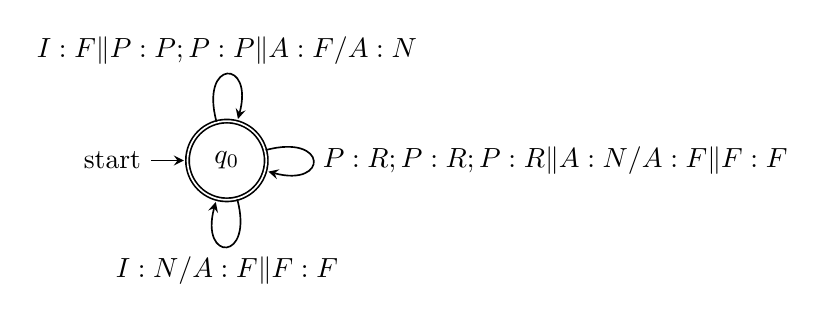
\begin{tikzpicture}[
    > = stealth,
    shorten > = 1pt,
    auto,
    node distance = 3cm,
    semithick
]

% Setup the styles for the states
\tikzstyle{accepting}=[double, draw=black, circle, minimum size=1cm]
\tikzstyle{state}=[draw=black, circle, minimum size=1cm]

% Draw the state
\node[state, initial, accepting] (q0) {$q_0$};

% Draw the transition (self-loop)
\draw (q0) edge[loop above] node{$I:F$$\|$$P:P;P:P$$\|$$A:F$/$A:N$} (q0);
\draw (q0) edge[loop right] node{$P:R;P:R;P:R$$\|$$A:N$/$A:F$$\|$$F:F$} (q0);
\draw (q0) edge[loop below] node{$I:N$/$A:F$$\|$$F:F$} (q0);

\end{tikzpicture}
\caption{mDSA of the Alarm EDT}
    \label{fig:state-diagram}
\end{figure}


%%The mDSA above is a succinct representation of the EDT semantics. The states of a multi-port DSA are defined as per the requirements of the system it models. For a system with internal variables $S_1,S_2,\dots$ with each variable $S_i$ having an alphabet $\Sigma_{S_i}$, the corresponding \mdsa has states $Q=\Sigma_{S_1} \times \Sigma_{S_2} \times \dots$, but as seen earlier, this can be captured using additional tape instead. The additional tapes $B_{S_1}, B_{S_2}, \dots$ are for the internal variables used in the system. These variables can read input as well as produce output, over the alphabet representing their state space. %For example, a variable $S_i$ has an alphabet $\Sigma_{S_i}$ with letters that can be input as well as output.
%%
%%Transitions must then be enhanced in our semantics i.e. a transition can now require the local variables $S_1, S_2,\dots$ to have values $(s_1, s_2 \dots)$  for it to match. When triggered, the values then change to $(s'_1,s'_2,\dots)$. Assume each variable $S_i$ has its corresponding tape labeled $B_{S_i}$%(we relabel the tapes $B_{k+1}, B_{k+2}, \dots, B_{k'}$ appropriately)
%%. Let us use the syntax $\langle (s_1, s_2 \dots), (u_1, \dots, u_k), (s'_1,s'_2,\dots) \rangle$ to represent this.
%%
%%\begin{enumerate}
%%\item A transition (with label $j$) $\langle (s_1, s_2 \dots), (u_1, \dots, u_k), (s'_1,s'_2,\dots) \rangle$ is matched if each $B_i (i\le k)$ has $u_i$ as suffix, the last letter of each $B_{S_i}$ is $s_i$, and either $H_{i}^{j}$ is at the end or the entire $u_i$ is after $H_{i}^{j}$. Additionally, at least one tape is non-empty after $H_{i}^{j}$.
%%
%%\item A matched transition is then triggered, moving each $H_{i}^{j}$-head of $B_i$ (or $B_{S_i}$) to the end. Additionally $\forall s'_i \ne \epsilon$, the corresponding $B_{S_i}$ extends by one position to the right and stores $s'_i$.
%%\end{enumerate}
%%
%%\textcolor{red}{Semantics for Row sequences}
%%We introduce the notion of a multi-transition, a transition with multiple parts that must occur in sequence. Let us illustrate with a two-part transition $\langle (s_1, s_2 \dots), (u_1, \dots, u_k), (s'_1,s'_2,\dots)$ ; $(s''_1, s''_2 \dots), (u'_1, \dots, u'_k), (s'''_1,s'''_2,\dots) \rangle$. For it to match, each $B_i (i\le k)$ must have $u_i  u'_i$ as suffix, each $B_{S_i}$ has $s_i  s''_i$, and either $H_{i}^{j}$ is at the end or the entire $u'_i$ occurs after $H_i^j$. Additionally, at least one tape is non-empty after $H_i^j$ heads. Not only this, all of $(s''_1, s''_2 \dots), (u'_1, \dots, u'_k)$ must occur after $(s_1, s_2 \dots), (u_1, \dots, u_k)$. That is each for any $i,j$ we have $u'_i$ and $s''_i$ appearing after $u_j$ and $s_j$. When the matched transition is triggered, the tapes and their head positions are updated as earlier.
%%
%%\textcolor{red}{TODO: Reachability for mDSA vs Test generation for EDT. Complexity result (possibly PSPACE-complete)}
%%
%\input{basic.tex}


%%% Local Variables:
%%% mode: latex
%%% TeX-master: "mDSA"
%%% End:


\section{Test generation}
\label{sec:test-generation}

% What is test generation? The decision problem
Given an EDT $\Tt$ and a row $R$ of $\Tt$ as input, the \emph{test
  generation problem} is to decide if there exists an execution
$\pi \in \Ll(\Tt)$ such that $R$ is triggered in $\pi$.
%
The problem is
intrinsically difficult: one might have to match an intermediate row
multiple times in order to generate a test case for $R$, in fact this
number could even be exponential. This is witnessed in the EDT that
implements an $n$ bit counter. In order to match a row with $n$ ones,
the row with $0$ followed by $(n-1)$ $1$ needs be matched $2^{n-1}$
times. 
%

\begin{theorem}
  \label{thm:test-generation-PSPACE}
  Test generation for EDTs is $\PSPACE$-complete.
\end{theorem}

We prove below that test generation is $\PSPACE$-complete

For an EDT, its mDSA has exponentially many
configurations of tapes. But each configuration requires polynomially many bits (the tapes themselves). Detecting a test
case amounts to non-deterministically guessing a sequence of configurations. By standard complexity arguments, this gives a
$\PSPACE$-upper bound. %As we saw, all other EDTs can be converted in polynomial time to basic EDTs.

For the hardness, we reduce the problem of DFA
intersection. Consider $n$ DFA $\Aa_1, \Aa_2, \dots, \Aa_n$. The
problem is to decide if their intersection is empty. Each $\Aa_i$
can be considered as an EDT with row sequences. Assume that the sets
of states are mutually disjoint. Add a binary local variable $l_i$ and rules
such that $l_i = 1$ if ``current'' state of $\Aa_i$ is accepting and
otherwise $l_i = 0$. Add a row $\Land_i l_i = 1 \imp U$ for some
update. This row matches iff there is a non-empty intersection.

\section{Experiments}
\label{sec:experiments}
A testsuite $\Pi(\Tt)$ for an EDT $\Tt$ is a set of executions such
that for each row $R$ of $\Tt$ there exists an execution
$\pi \in \Pi$ and $\pi$ triggers $R$. To find a testsuite, we need to solve the test generation problem for each row.
%The testsuite generation problem is to check whether there exists a testsuite for a given EDT.

We have developed a prototype tool that implements an
algorithm to solve the test generation problem by systematically
exploring the configurations of an mDSA corresponding to the given EDT,
$\Tt$.  %The tool does not handle timing.

We conducted experiments to validate the following:

\begin{enumerate}
\item For simple EDTs, the tool can find test cases succesfully.
\item There are some EDTs for which it can solve the test
  generation problem, where randomized techniques (likely) cannot.
\end{enumerate}

%\texttt{Random} uniformly samples a set of executions, $\Pi_R(\Tt)$, of size
%$N$, from the universal set of executions that have exactly $P$ inputs
%and checks whether $\Pi_R(\Tt)$ is a testsuite for $\Tt$. \texttt{RGRaF}, on
%the other hand, employs a heuristic to sample a set of executions of
%size $N$ and checks whether it is a testsuite. \texttt{RGRaF} takes a parameter
%$P$ to restrict the number of inputs in each execution.

First we look at a couple of small EDTs. Table~\ref{tab:alarm-2} gives an example motivated from
\cite{Venkatesh:ENASE:2015} which describes selected requirements of a
car alarm module. It is similar to Table~\ref{tab:edt-alarm} from Section~\ref{sec:edt}. Encoding this in our tool gives a testcase (Press; Press) for Row 1.

\begin{table}[h!]
  \centering \def\arraystretch{1.2}
  \caption{EDT for an Alarm module}
  \label{tab:alarm-2}
  \begin{tabular}{|c|c|c|c||c|c|}
    \hline
    sno & \specialcell{in \\ Ignition} &
                                         \specialcell{in \\ PanicSw} &
                                                                       \specialcell{in 
    \\ Alarm} & \specialcell{out \\ Alarm} & 
                                             \specialcell{out \\ Flash} \\
    \hline 
    1 & Off & (Press; Press)%\{$<1$s\} 
    & Off & On &
    \\
    \hline

    2 & On & & & Off & False \\
    \hline
  \end{tabular}
  
\end{table}

Next we look at Table~\ref{tab:wiper}, a partial representation of a wiper module in a car. The tool finds a testcase for Row 2.

\begin{table}[h!]
  \centering \def\arraystretch{1.2}
  \caption{EDT for a Wiper module}
  \label{tab:wiper}
  \begin{tabular}{|c|c|c|c|c||c|c|}
    \hline
    sno & \specialcell{in \\ ignition} &
                                         \specialcell{in \\ wiperswitch} & 
                                                                       \specialcell{in 
    \\ parksensor} & \specialcell{in \\ error} & \specialcell{out \\ wipercmd} & 
                                             \specialcell{out \\ error} \\
    \hline 
    1 & on & on & 
    & false & wipe &
    \\
    \hline

    2 & & & (park;notpark) & & dontwipe & true \\
    \hline
  \end{tabular}
  
\end{table}


For the other claim, we created a specific kind of EDT for
which the probability of randomized techniques selecting a required
execution is very low. The EDT extends the three bit counter,
shown in Table \ref{tab:binary}, to five bits and adds a 
row to reset the counter. Our tool solves this problem, and hence for rows that have a very low probability of getting triggered
it is better than randomized techniques.

%Table \ref{tab:binary} shows a counter for $3$ bits.

\begin{table}
  \centering
  \renewcommand{\arraystretch}{1.2} 
  \caption{Implementing a binary counter for $3$ bits}
  \label{tab:binary}
  \begin{tabular}{|c|c|c|c|c||c|c|c|c|}
    \hline
    $T$ & $t_2$ & $t_1$ &$t_0$ & $S_T$ & $t_2$ & $t_1$ & $t_0$ & $S_T$                                                             
    \\
    \hline
     \checkmark & & & & & & & & $+$  \\
         
    \hline
     & & & $0$ & $+$ & & & $1$ & $-$  \\

    \hline
   & & $0$ & $1$ & $+$ & & $1$ & $0$ & $-$ \\

    \hline
   & $0$ & $1$ & $1$ & $+$ & $1$ & $0$ & $0$ & $-$ \\

    \hline
  \end{tabular}
\end{table}


%%% Local Variables:
%%% mode: latex
%%% TeX-master: "m"
%%% End:

\section{Related Work}
Use of automata to model distributed systems has been explored widely.
Esterel~\cite{DBLP:journals/scp/BerryG92} is a synchronous programming language
that provides a parallel composition operator. Harel's
Statecharts!\cite{DBLP:journals/scp/Harel87} also support parallel composition
of state transition systems. In both these languages the reaction of a system
in response to inputs on each port can be specified separately and the
different specifications can be composed using the parallel operator. A system
model can then refer to the states of each port's specification to model the
system behaviour. System behaviours similar to the examples described in this
paper can be specified more succinctly using mDSAs. Petri nets~\cite{CAPetri}
have been studied extensively to model concurrent systems. In Petri nets each
letter of each port's alphabet will have to be represented using a place and
the places combined to model the system. This will not be as succinct as an
mDSA. 
The work that is closest to ours is Input/Output Partial Order
Automata(IOPOA)~\cite{10.5555/2391293.2391305}. In their work transitions
execute non-atomically reacting to asynchronous inputs on several ports. The main differences between IOPOA and mDSA are - in mDSA transitions react atomically, transition labels can be strings for each port and not just letters and different transitions may trigger on the same string at a port.


\section{Todos.}

\begin{itemize}
\item Compare the succinctness of mDSAs with DSAs. Understanding the
  effect of partitioning the alphabet and the automaton having the
  ability to treat them as independent events. We expect exponential
  succinctness easily, in terms of the number of input variables.

\item Comparison of mDSAs with streaming string transducers. Seem
  incomparable - the motivations are different. What about transducers
  with regular look ahead? 

\item Reachability of mDSAs: algorithm and a potential encoding in
  SAT?
  
\item EDTs to mDSAs: formal semantics for EDTs as mDSA. 

\item Test generation algorithm for EDTs reduced reachability in
  mDSAs. Complexity of test generation. 

\item Can we encode the test generation procedure as a SAT solving
  algorithm, instead of explicitly constructing the EDT and then
  running a reachability algorithm? This SAT-based solution should
  take an EDT and spit out a bunch of SAT queries, to cover each
  row. This also allows us to ask for ``bounded'' test case
  generation. 

\item Experiments. Give arguments to show that situation is better
  than before. Independently, is mDSA useful in a different
  setting. Potentially a new case study that illustrates the use of
  EDT methodology in a new setting.  
  
\end{itemize}

\bibliographystyle{splncs04}
\bibliography{mDSA}

\end{document}	
